% The document class supplies options to control rendering of some standard
% features in the result.  The goal is for uniform style, so some attention 
% to detail is *vital* with all fields.  Each field (i.e., text inside the
% curly braces below, so the MEng text inside {MEng} for instance) should 
% take into account the following:
%
% - author name       should be formatted as "FirstName LastName"
%   (not "Initial LastName" for example),
% - supervisor name   should be formatted as "Title FirstName LastName"
%   (where Title is "Dr." or "Prof." for example),
% - degree programme  should be "BSc", "MEng", "MSci", "MSc" or "PhD",
% - dissertation title should be correctly capitalised (plus you can have
%   an optional sub-title if appropriate, or leave this field blank),
% - dissertation type should be formatted as one of the following:
%   * for the MEng degree programme either "enterprise" or "research" to
%     reflect the stream,
%   * for the MSc  degree programme "$X/Y/Z$" for a project deemed to be
%     X%, Y% and Z% of type I, II and III.
% - year              should be formatted as a 4-digit year of submission
%   (so 2014 rather than the accademic year, say 2013/14 say).
%
% Note there is a *strict* requirement for the poster to be in portrait 
% format so that we display them on the poster boards available.

\documentclass[]{templates/poster}

\usepackage{pifont}
\usepackage{caption}
\usepackage{subcaption}
\usepackage{graphicx}
\usepackage{amsthm}
\usepackage{wrapfig}
\usepackage{framed}

\DeclareGraphicsExtensions{.pdf}

\postertitle{Quantum speedup of the Travelling Salesman Problem for bounded-degree graphs}
\posterauthors{Dominic J. Moylett\textsuperscript{1,2,3}, Noah Linden\textsuperscript{4} and Ashley Montanaro\textsuperscript{4}}
\posteraffils{\textsuperscript{1}Quantum Engineering Technology Labs, University of Bristol\\\textsuperscript{2}Quantum Engineering Centre for Doctoral Training, University of Bristol\\\textsuperscript{3}Heilbronn Institute for Mathematical Research, University of Bristol\\\textsuperscript{4}School of Mathematics, University of Bristol}

\begin{document}

% -----------------------------------------------------------------------------

\begin{frame}{} 

\begin{columns}[t]
  \begin{column}{0.900\linewidth}
  \begin{block}{\Large Introduction and Main Results}
  The Travelling Salesman Problem (TSP) is one of the oldest and most famous problems in graph theory. It is known that any classical algorithm for exactly solving the problem must take superpolynomial time unless $P = NP$. But little research has been undertaken on determining whether or not quantum algorithms can outperform classical algorithms for this problem.
  
  We demonstrate near-quadratic speedups for solving the TSP when the degree of any vertex in the graph is at most $4$. This is through applying a quantum speedup for backtracking algorithms developed by Montanaro [Mon15] to a pair of algorithms by Xiao \& Nagamochi [XN16a,XN16b] for solving the TSP. We then demonstrate polynomial speedups for graphs of higher degrees. 
  
  See {\tt arXiv:1612.06203} for more information.
  \end{block}
  \end{column}
\end{columns}

\begin{columns}[t]
  \begin{column}{0.422\linewidth}
  \begin{block}{\Large 1. The Travelling Salesman Problem}
  Let $G = (V, E)$ be a graph with $n$ vertices $V$ and $m$ edges $E$. Associated with $G$ is a cost function $C \colon E \rightarrow \mathbb{Z}^+$. A cycle $H$ on $G$ is a {\em Hamiltonian cycle} if it visits every vertex in $G$ exactly once. The Travelling Salesman Problem is to return the minimum cost Hamiltonian cycle.
  
  \begin{center}
  \begin{figure}
  \begin{subfigure}[t]{0.3\linewidth}
  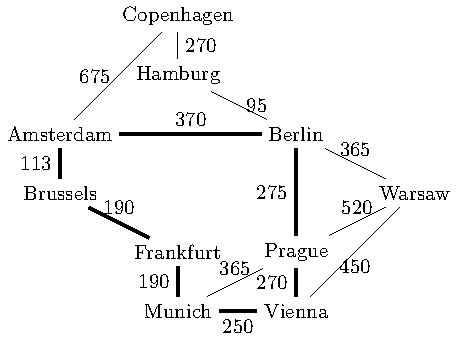
\includegraphics[width=\linewidth]{not_hamiltonian}
  \caption{\ding{55} Not a Hamiltonian cycle.}
  \end{subfigure}
  \begin{subfigure}[t]{0.3\linewidth}
  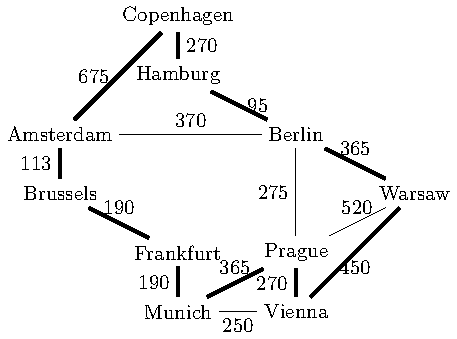
\includegraphics[width=\linewidth]{not_shortest}
  \caption{\ding{55} Not the shortest Hamiltonian cycle. (Length: $2983$ Minutes)}
  \end{subfigure}
  \begin{subfigure}[t]{0.3\linewidth}
  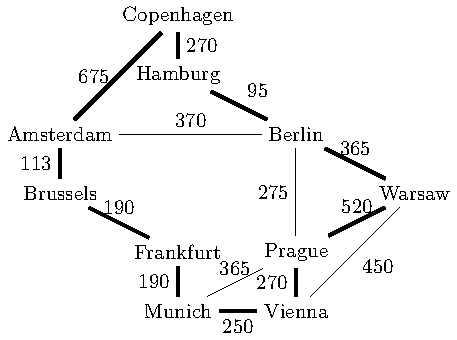
\includegraphics[width=\linewidth]{shortest}
  \caption{\ding{51} Solution to the Travelling Salesman Problem. (Length: $2938$ Minutes)}
  \end{subfigure}
  \end{figure}
  \end{center}
  \end{block}

  \begin{block}{\Large 2. Backtracking algorithms}
  Backtracking algorithms are a way of solving constraint satisfaction problems faster than na\"ive search. This is done using a predicate $P$, which checks if a partial assignment might satisfy the constraints, and a heuristic $h$, which recommends the next variable to assign given a partial assignment.
  
  Montanaro [Mon15] demonstrated a quantum backtracking algorithm which has a quadratic speedup in the number of calls to $P$ and $h$ for finding any solution. This is under the constraints that the predicate and heuristic only depend on local information and that the entire backtracking algorithm's search space is explored.
  \end{block}
  \end{column}

  \begin{column}{0.422\linewidth}
  \begin{block}{\Large 3. Quantum speedup of the TSP for degree-3 graphs}
  Backtracking algorithms for the TSP solve the problem of finding the shortest Hamiltonian cycle that includes a subset of ``forced'' edges. The predicate checks whether or not such a Hamiltonian cycle is still possible, and the heuristic selects another edge to either force or remove from the graph. This continues until a Hamiltonian cycle is found, a Hamiltonian cycle is impossible to find, or the graph is such that the TSP can be solved in polynomial time via [Epp07, Lemma 3].

  The best-performing backtracking algorithm for the TSP on degree-3 graphs is the Xiao-Nagamochi algorithm, which runs in $O^*(2^{3n/10})$ time and polynomial space, where $O^*$ hides polynomial factors.
  
  The details of the Xiao-Nagamochi algorithm are technical, but the steps the algorithm takes can be broken up into a predicate, a heuristic and a reduction function, where the reduction function is a step called by both the predicate and heuristic to simplify the graph.

  By applying the quantum speedup from [Mon15] to the Xiao-Nagamochi algorithm, we can find a Hamiltonian cycle with failure probability $\delta$ in $O^*(2^{3n/20}\log(1/\delta))$ time.
  
  To find the shortest Hamiltonian cycle, we repeat the algorithm but add the constraint that the length of the cycle must be shorter than a given bound. We update this bound in a binary search fashion, and find the shortest Hamiltonian cycle in $O^*(2^{3n/20}\log L\log\log L)$ time, where $L$ is the length of the longest edge and the $\log\log L$ term is to make the probability of error arbitrarily small.
  \end{block}
  \end{column}
\end{columns}
  
  \begin{columns}[t]
  \begin{column}{0.422\linewidth}

  \begin{block}{\Large 4. Expanding to higher-degree graphs}
  \begin{wrapfigure}[11]{r}{0.2\linewidth}
  \begin{framed}\raggedleft
  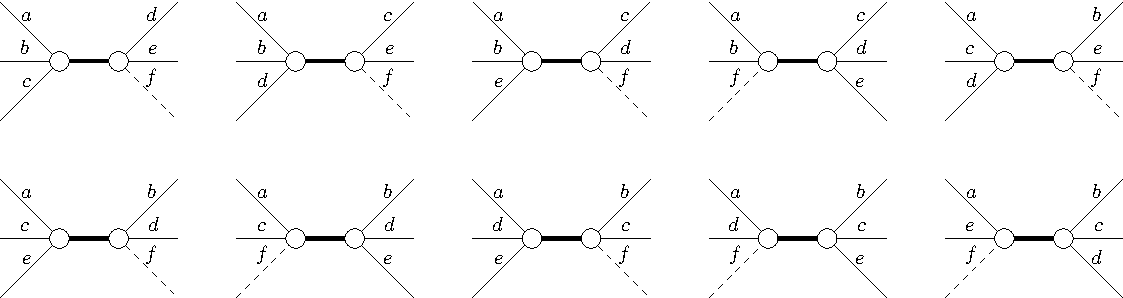
\includegraphics[width=\linewidth]{deg5}
  \caption{Example of splitting a vertex of degree 6 into two vertices of degree 4.}
  \end{framed}
  \end{wrapfigure}

  For degree-4 graphs, we apply the speedup from [Mon15] to the algorithm of [XN16b], solving the problem in $O^*(1.301^n\log L \log\log L)$ time.
  
  Speedups for graphs of degree 5 and 6 can be found by breaking higher-degree vertices into degree-4 vertices connected by a forced edge. We use D\"urr and H\o yer's minimum-finding algorithm [DH99] to search over possible ways of splitting each vertex and return the minimum.
  
  If there are $f$ vertices of degree $5$ or $6$, there are $10^f$ splittings, of which $6^f$ will succeed. Our runtime is  $O^*((10/6)^{f/2}1.301^n\log L\log\log L) = O^*(1.680^n\log L\log\log L)$.

  At degree-7, classical algorithms for the general TSP are faster [HK62, Bj\"o14].
  \end{block}
  \end{column}

  \begin{column}{0.422\linewidth}
  \begin{block}{\Large References}
  [Bj\"o14] A. Bj{\"o}rklund, SIAM Journal on Computing, 43(1):280--299 (2014)

  \noindent[DH99] C. D\"urr and P. H\o yer, {\tt arXiv:quant-ph/9607014} (1999)

  \noindent[Epp07] D. Eppstein, Journal of Graph Algorithms and Applications, 11(1):61--81, (2007)

  \noindent[HK62] M. Held and R. Karp, Journal of the Society for Industrial and Applied Mathematics, 10(1):196--210, (1962)

  \noindent[Mon15] A. Montanaro, {\tt arXiv:1509.02374} (2015)

  \noindent[XN16a] M. Xiao and H. Nagamochi, Algorithmica 74(2):713--741, (2016)

  \noindent[XN16b] M. Xiao and H. Nagamochi, Theory of Computing Systems, 58(2):241--272, (2016)
  \end{block}
  \end{column}
\end{columns}

\end{frame}

% -----------------------------------------------------------------------------

\end{document}



